\documentclass[12pt]{article}

\usepackage{tocloft}
\usepackage[margin=0.5in]{geometry} %used for margins
\usepackage{graphics}
\usepackage{graphicx}
\usepackage{gensymb} %for symbols such as the degree sign
\usepackage{titlesec}
\graphicspath{
{figures/}
}
\usepackage[natbibapa]{apacite}
% \usepackage[]{natbib}
\usepackage{xcolor}
\usepackage{array}% http://ctan.org/pkg/array
\usepackage{tikz} %used for drawing colored boxes 
\usepackage{bibentry} %for full citations
% \nobibliography* 
\usepackage{subfig} %for creating panels
\usepackage{todonotes}  
\usepackage{booktabs}% http://ctan.org/pkg/booktabs
\usepackage{ctable}% http://ctan.org/pkg/booktabs
\usepackage[countmax]{subfloat} %for creating panels
\usepackage{enumitem} %better environment for lists 
\usepackage{multirow} %to have multiple row entries in tables 
\usepackage{breakurl} %to break urls
\usepackage{wrapfig} %to wrap figures
\usepackage{float}  %for floating figures
\usepackage{amsmath}
\usepackage{hyperref} %to h ave links within the document
\usepackage{placeins}

\hypersetup{
    colorlinks,%
    citecolor=black,%
    filecolor=black,%
    linkcolor=black,%
    urlcolor=black
}

%to allow for more figures per page 
\renewcommand\floatpagefraction{.95}
\renewcommand\topfraction{.95}
\renewcommand\bottomfraction{.95}
\renewcommand\textfraction{.05}   
\setcounter{totalnumber}{50}
\setcounter{topnumber}{50}
\setcounter{bottomnumber}{50}

%some settings to make lists look nicer 
\setlist{leftmargin=*} 
\setlist[1]{labelindent=\parindent} % Only the level 1
\setlist{topsep = 0cm,partopsep = 1pt, parsep = 1pt} %changes the separation of lists 

%some stuff to decrease the space around section headings, etc. 
\titleformat{\section}
  {\bfseries \Large}{\thesection}{0.5em}{}

\titleformat{\subsection}
  {\bfseries \large}{\thesubsection}{0.5em}{}

\titleformat{\subsubsection}
{\bfseries}{\thesubsubsection}{0.5em}{}

\titlespacing{\section}{0cm}{0.3cm}{0.1cm}
\titlespacing{\subsection}{0cm}{0.3cm}{0.1cm}
\titlespacing{\subsubsection}{0cm}{0.3cm}{0.1cm}


\newcommand{\ttodo}[2][]
{\todo[caption={#2}, size=\small, #1, color = green, inline]{\renewcommand{\baselinestretch}{1}\selectfont \textbf{TG}: #2}~}

\newcommand{\ntodo}[2][]
{\todo[caption={#2}, size=\small, #1, color = yellow, inline]{\renewcommand{\baselinestretch}{1}\selectfont \textbf{NB}: #2}~}

\newcommand{\rtodo}[2][]
{\odo[caption={#2}, size=\small, #1, color = blue, inline]{\renewcommand{\baselinestretch}{1}\selectfont \textbf{RM}: #2}~}

\newcommand{\sntodo}[2][]
{\todo[size=\footnotesize, color = yellow, #1]{#2}~}

\DeclareMathOperator*{\Do}{Do}
\DeclareMathOperator*{\pa}{pa} %Parents

\newcommand{\ww}{\mathbf{w}} %Parameter
\newcommand{\ws}{w_S} %Parameter
\newcommand{\wb}{w_B} %Parameter

\newcommand{\mm}{m} %Single causal model
\newcommand{\mmm}{M} %Random variable causal models
\newcommand{\cald}{\mathcal{D}} %Set of data
\newcommand{\calc}{\mathcal{C}} %Set of interventions
\newcommand{\calm}{\mathcal{M}} %Set of models

\newcommand{\ci}{\mathbf{c}} %Single intervention
\newcommand{\ccc}{C} %Set of interventions
\newcommand{\da}{\mathbf{d}} %Data

\DeclareMathOperator*{\zz}{\mathbf{z}} %Actual causation
\DeclareMathOperator*{\zzz}{\mathbf{Z}} %Actual causation


\begin{document}

\begin{center} 
{\LARGE \textbf{Time intervene cycles notes}}
\linebreak
\linebreak
{\large Neil Bramley (\href{mailto:neil.bramley@ucl.ac.uk}{neil.bramley@ucl.ac.uk})}
\linebreak
\today
\end{center} 

\section{Experiment 1 results}

\FloatBarrier

\subsection{Judgments: Normative inference or incremental construction?}


\begin{itemize}
  \item Judgment accuracy is lower for cyclic models while 'normatively' there is more information.  This hints at cognitive constraints...
  \item No relationship between entropy/information/ideal-accuracy and actual accuracy!
  \item Interaction between number of effects, cyclicity and accuracy.  Participants do better when they see more effects in acyclic systems and less effects in cyclic systems.
  \item Satisfyingly, the \emph{most recent} heuristic is terrible at forks
\end{itemize}

\begin{figure}[H]
   \centering
   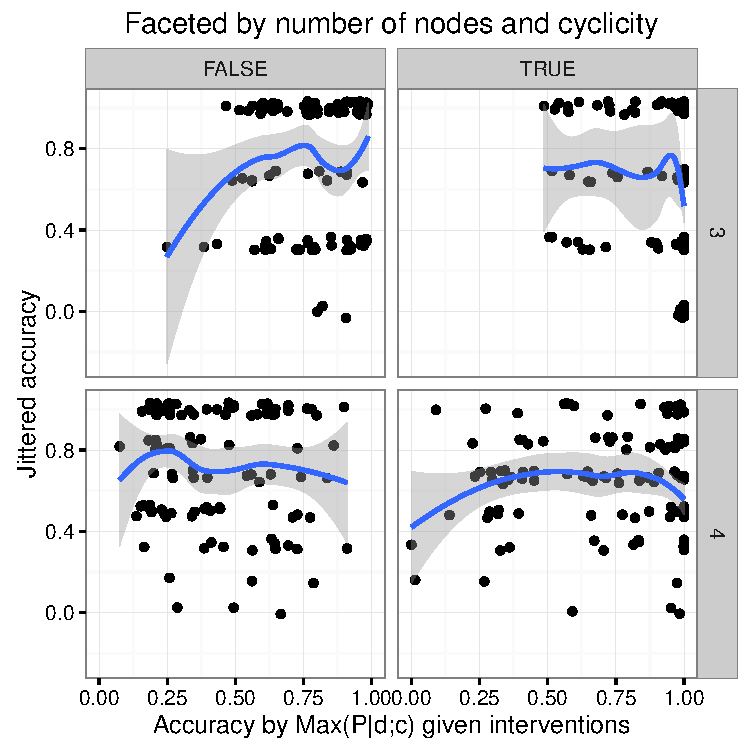
\includegraphics[width = .5\columnwidth]{information_accuracy_relationship}
   \caption{example caption}
   \label{fig:information_accuracy_relationship}
\end{figure}

\begin{figure}[H]
   \centering
   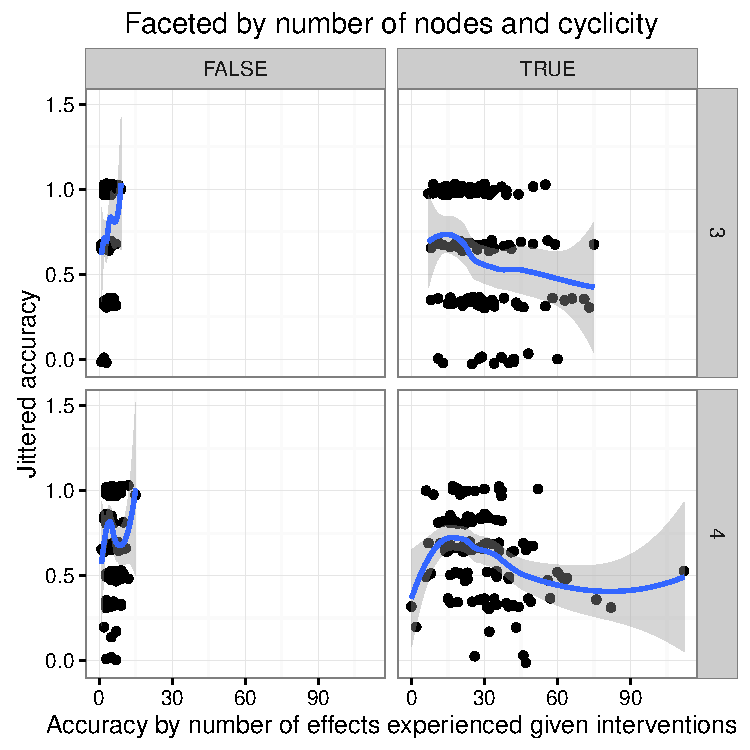
\includegraphics[width = .5\columnwidth]{n_effects_accuracy_relationship}
   \caption{example caption}
   \label{fig:n_effects_accuracy_relationship}
\end{figure}

\begin{figure}[h]
   \centering
   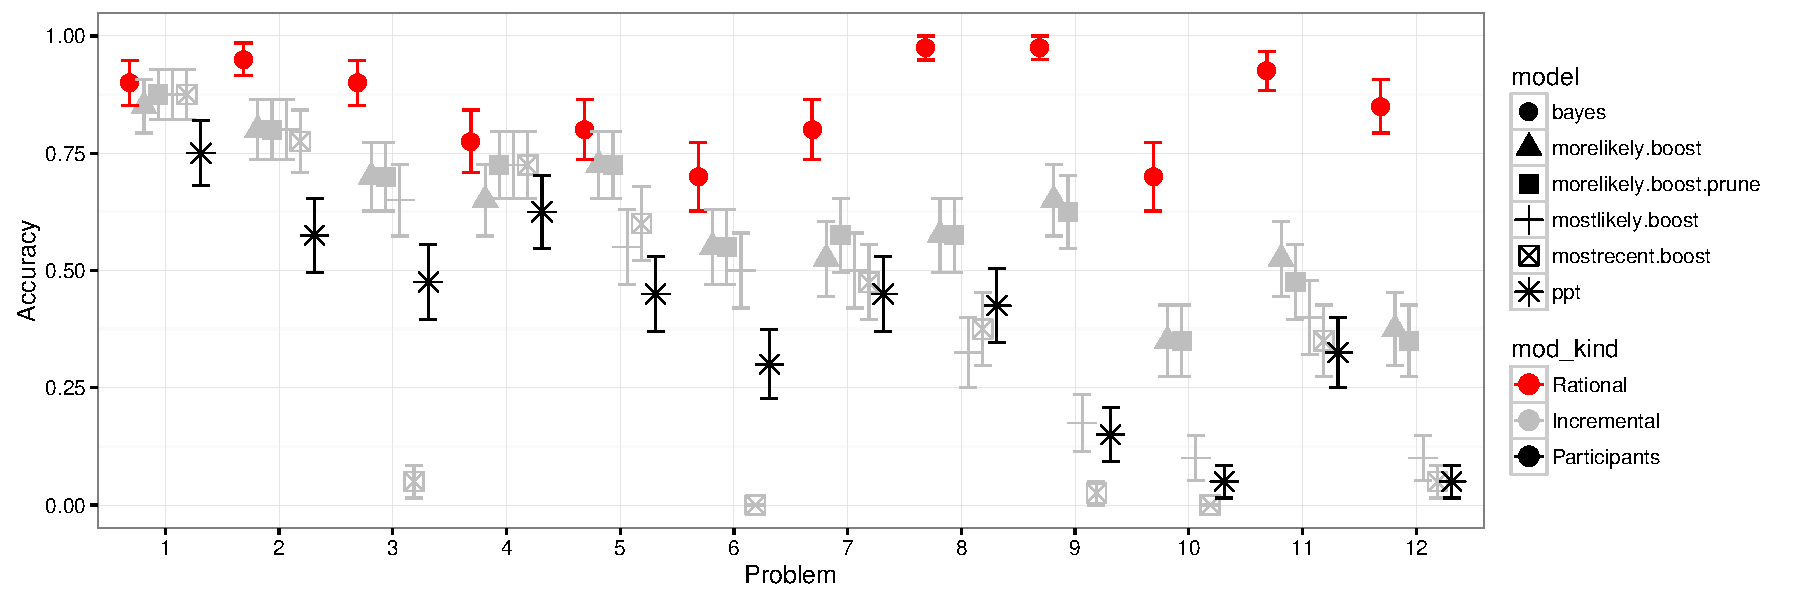
\includegraphics[width = \columnwidth]{ppt_mod_pcorrect_trial}
   \caption{Participants' proportion correct compared to Rational responding and Incremental heuristics}
   \label{fig:ppt_mod_pcorrect_trial}
\end{figure}

\begin{figure}[h]
   \centering
   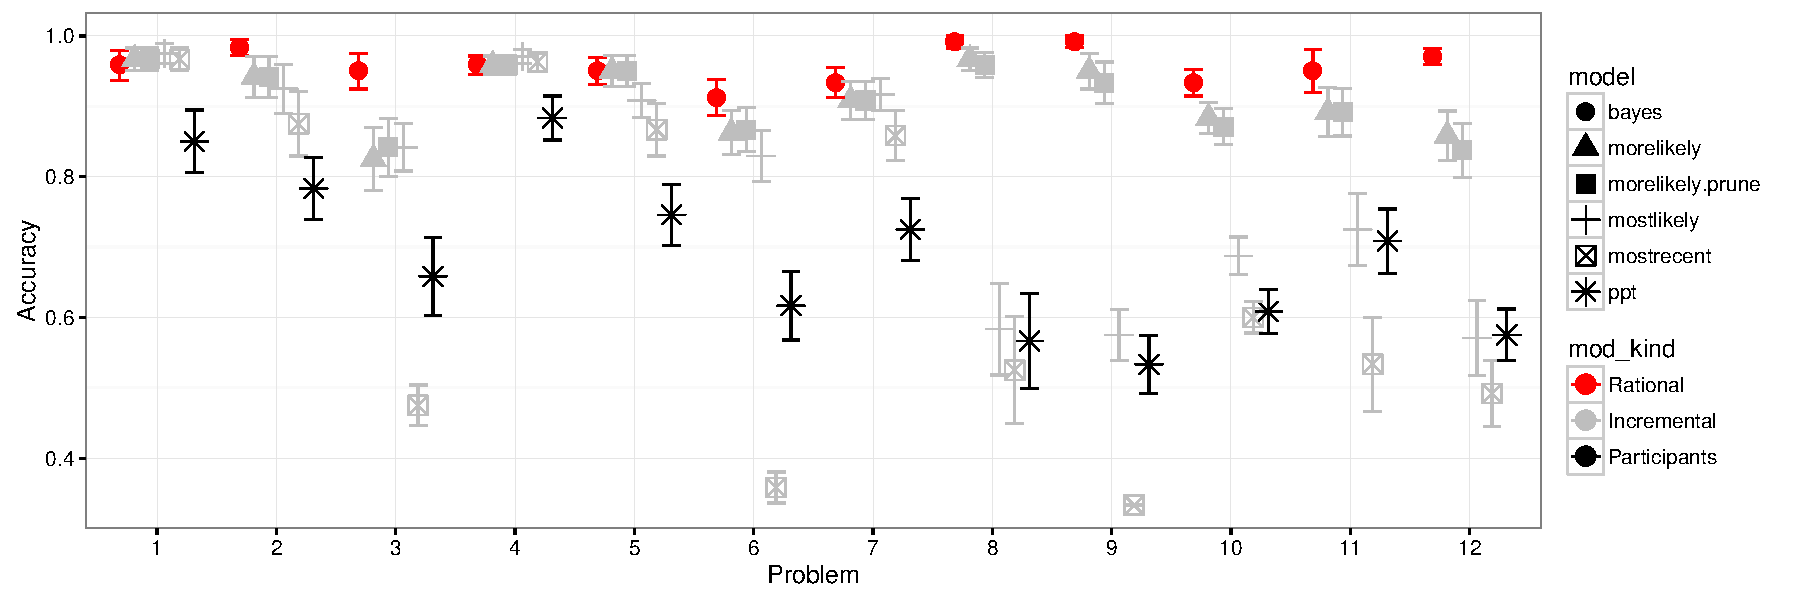
\includegraphics[width = \columnwidth]{ppt_mod_performance_trial.pdf}
   \caption{Participants' (edgewise) accuracy compared to Rational and incremental responding}
   \label{fig:ppt_mod_performance_trial.pdf}
\end{figure}



\begin{table}[ht]
\centering
\caption{Model comparison}
\label{table:incremental_construction}
\footnotesize{
\begin{tabularx}{\columnwidth}{lXXXXXX}
\toprule
Model & \multicolumn{2}{l}{Accuracy (\%)}  & \multicolumn{2}{l}{Accordance (\%)}  & \multicolumn{2}{l}{N best (/60)}  \\ 
 & All & Final & All & Final & All & Final\\
\hline
Random & 25 & 25 & 25 & 25 & 0 & 0 \\
Most recent & 66.2 & 64.7 & 67.2 & 64.9 & 16 & 17 \\ 
  Most likely & 79.7 & 78.9 & 67.3 & 65.5 &  4 &  5 \\ 
  More likely & 87.9 & 90.9 & 69.3 & 69.2 & 13 & 12 \\ 
  More likely + Pruning & 87.6 & 90.5 & 69.5 & 69.4 &  3 &  2 \\ 
  Rational & 91.0 & 95.3 & 66.1 & 68.9 &  4 &  4 \\ 
   \bottomrule
\end{tabularx}}
\footnotesize{\emph{Note:} ``Best'' determined by the greatest proportion matching connections across judgments).}\raggedright
\end{table}

\FloatBarrier


\subsection{Comparison with simulated interventions}
\ntodo{New stuff}

\begin{itemize}
  \item Participants interventions are great, they are better than the simulations'
\end{itemize}



\begin{figure}[h]
   \centering
   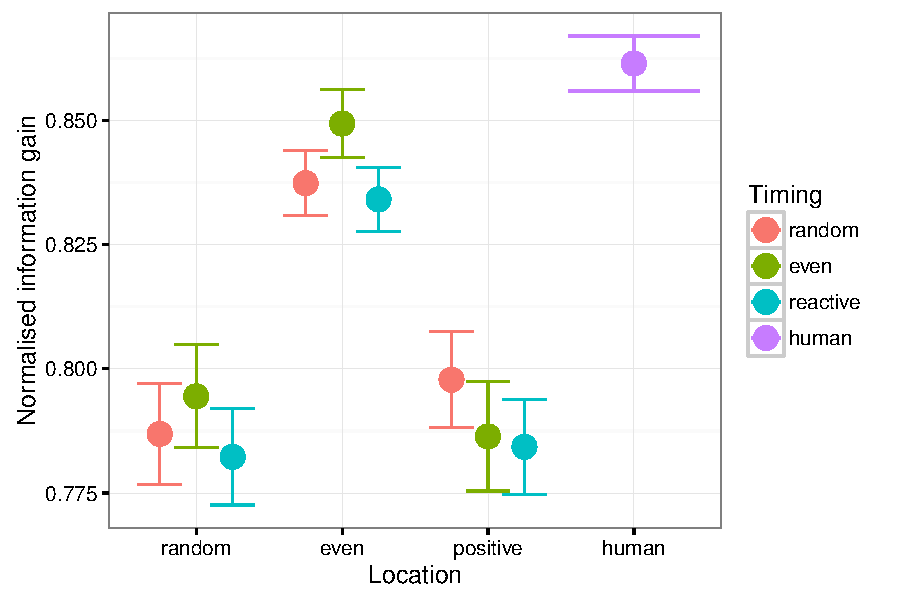
\includegraphics[width = .5\columnwidth]{int_sim_performance}
   \caption{Performance of intervention heuristics compared to participants' choices}
   \label{fig:int_sim_performance}
\end{figure}


\begin{figure}[h]
   \centering
   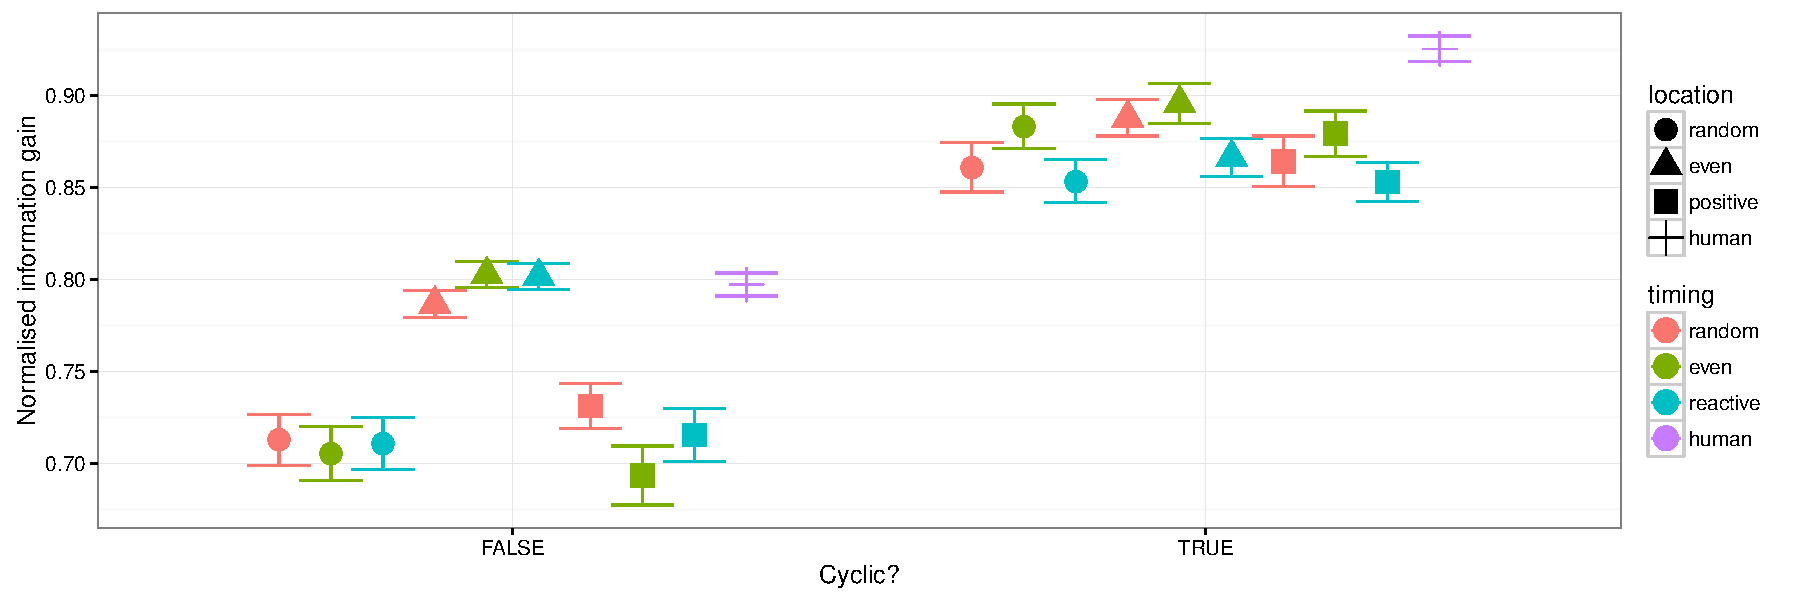
\includegraphics[width = \columnwidth]{int_sim_performance_cyclic}
   \caption{Performance of intervention heuristics compared to participants' choices, split by acyclic/cyclic.}
   \label{fig:int_sim_performance_cyclic}
\end{figure}

\begin{figure}[h]
   \centering
   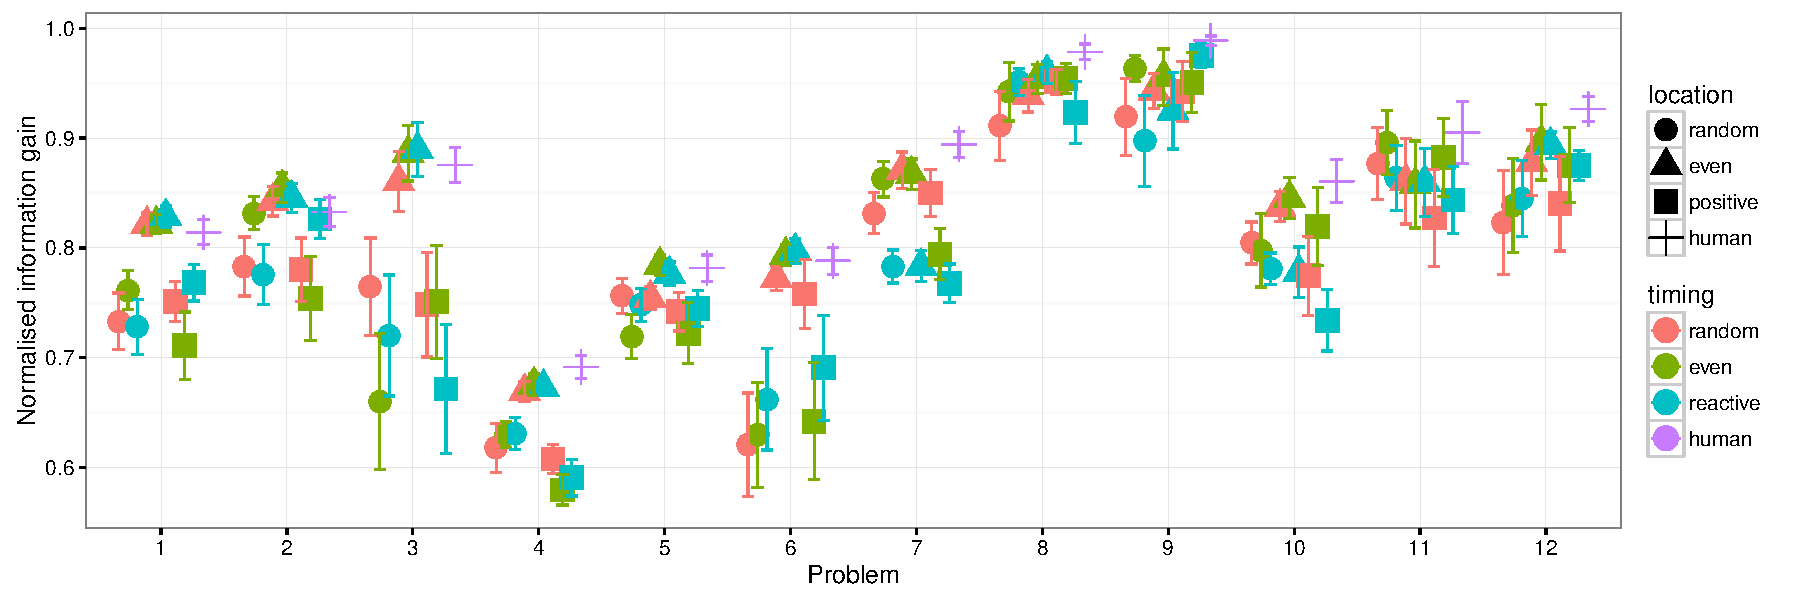
\includegraphics[width = \columnwidth]{int_sim_performance_trial}
   \caption{Performance of intervention heuristics in terms of normalised information gain compared to participants' choices, split by device}
   \label{fig:int_sim_performance_trial}
\end{figure}


\begin{figure}[h]
   \centering
   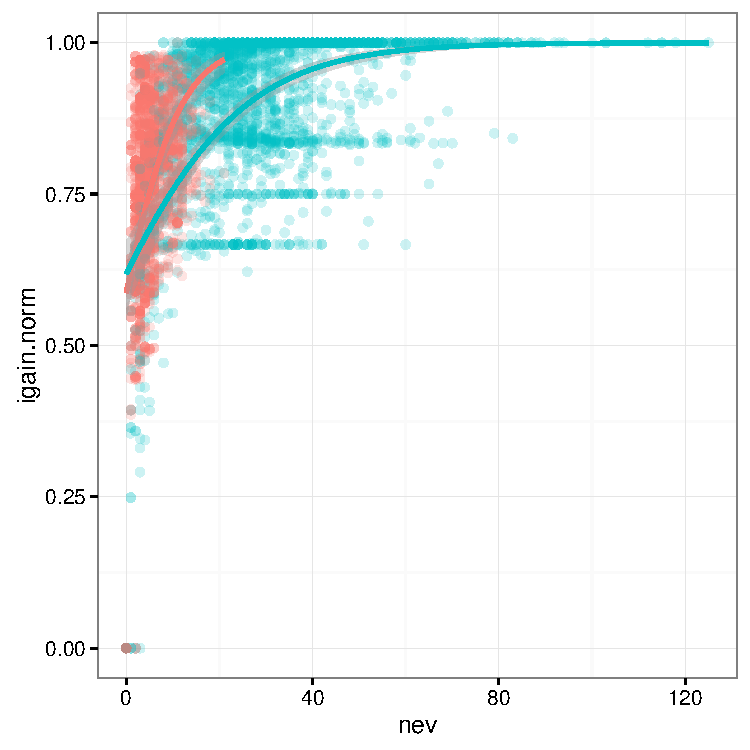
\includegraphics[width = .48\columnwidth]{nev_igain_correlation}
   \caption{Relationship between the number of events and the information obtained (measured by the $\max P(M|\mathbf{d};\mathbf{c})$}
   \label{fig:nev_max_p_correlation}
\end{figure}

\FloatBarrier

\subsubsection{Distributions of delays between interventions and preceding events/interventions}

\begin{figure}[h]
   \centering
   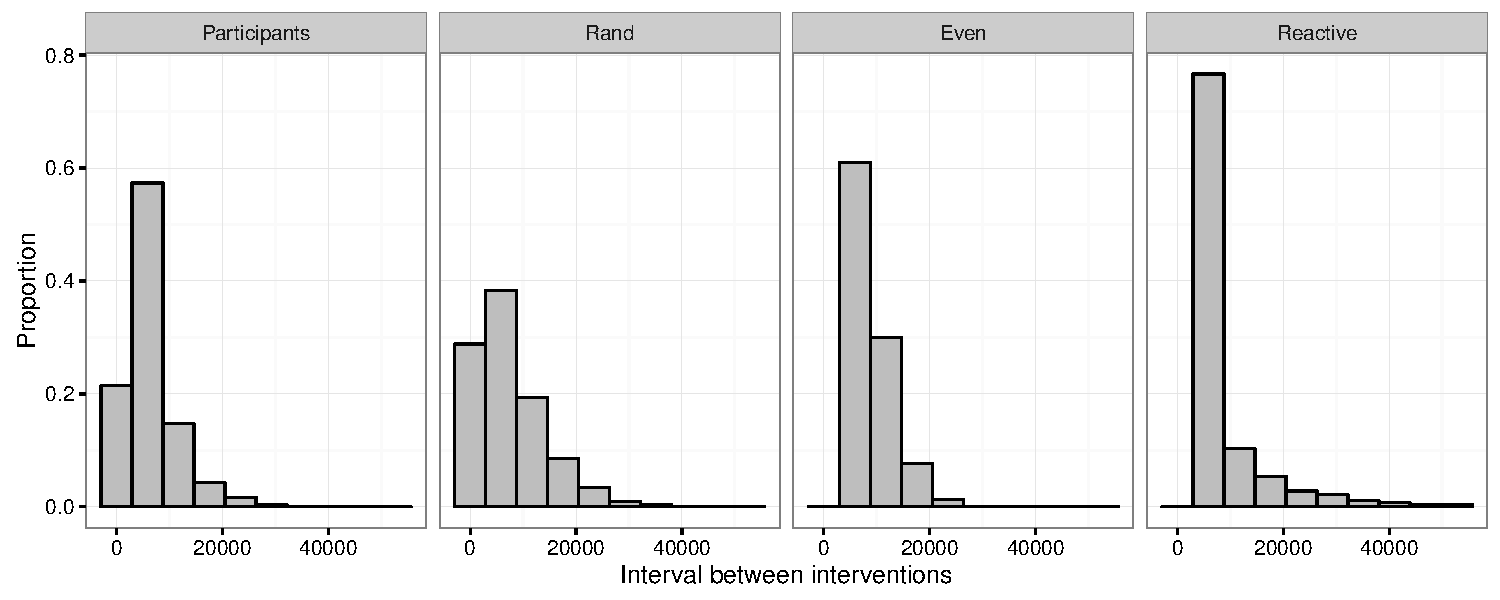
\includegraphics[width = \columnwidth]{interintervention_intervals}
   \caption{Intervals between interventions for participants and simulations}
   \label{fig:interintervention_intervals}
\end{figure}

\begin{figure}[h]
   \centering
   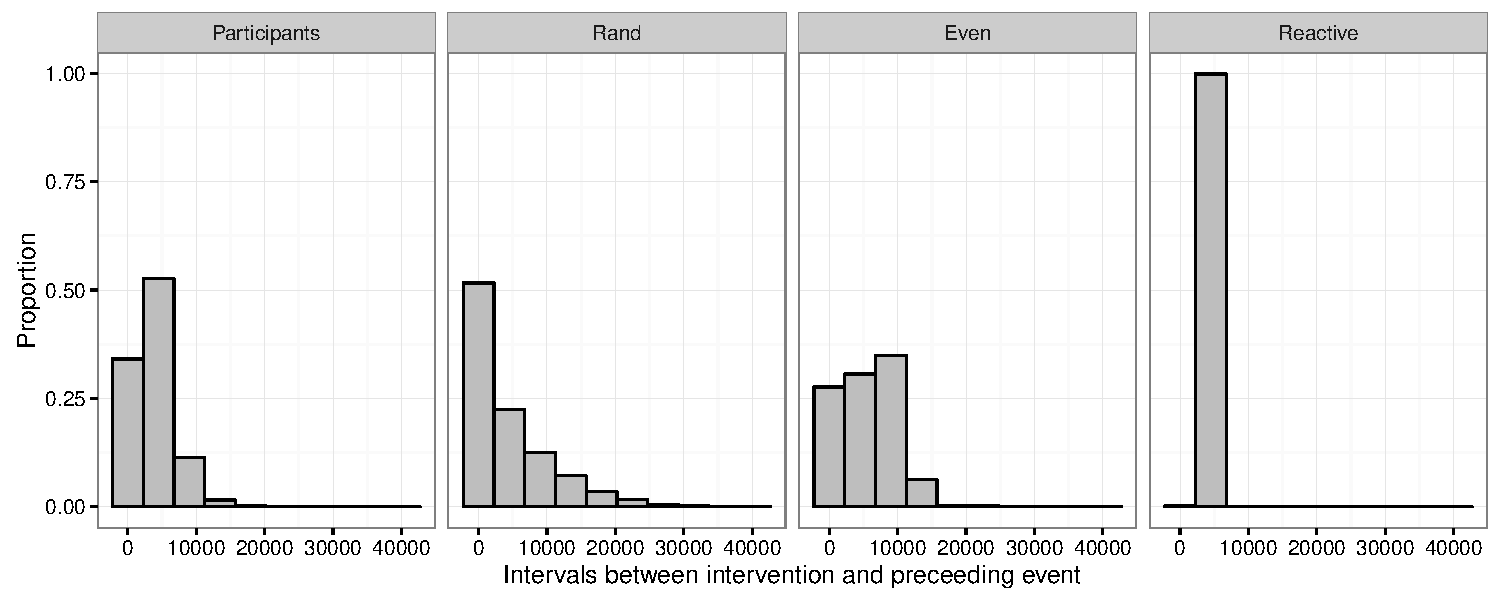
\includegraphics[width = \columnwidth]{reaction_intervals}
   \caption{Intervals between interventions and the most-recently-preceeding events for participants and simulations}
   \label{fig:reaction_intervals}
\end{figure}




\bibliography{../cogsci_paper/refs}

\end{document}